\section{Introduction}

Bubbles within liquids are incredibly common, occurring in both a wide spectrum of natural and industrial processes \cite{Volcano,bird2010daughter,deike2022mass,dollet2019bubble,feng2014nanoemulsions,oratis2020new,veron2015ocean,WINE}. These occurrences can range from water and carbon-dioxide bubbles in magma providing driving forces for an eruption \cite{Volcano} to carbon-dioxide bubbles in champagne enhancing the evaporation of volatile organic compounds dispersed in the liquid phase. When a bubble rises to the surface of a liquid, it may burst, scattering many droplets. These droplets are an important process of transport exchange across the liquid gas interface\cite{notdoneyet}, they are considered the main source of sea spray aerosols and impact air pollution[] as well as the transmission of infectious diseases[]. Bubbles formed due to the breaking of waves contribute to the transfer of heat, mass and other contaminants between the oceans and the atmosphere. The efficiency of this transfer is governed by the initial size and speed of the ejected drops.

There are two Phenomena that occur when a bubble bursts that produce aerosols, the first being when the thin film separating the bubble from the atmosphere is ruptured. The atomisation of the film can produce several hundred droplets of around a micrometer in diameter. Due to the length scales of the rupture being order O($100$nm), we are unable to describe this problem with continuum mechanics. In fact, van der Waals forces or electrostatic repulsion must be considered, both of which are long-range intermolecular forces.

After the film rupture, the remaining cavity collapses causing a jet to form. This jet eventually breaches into one or more droplets. The key difference between these droplets and the droplets formed when the film ruptures is that they are much larger, order O($100 \mu$m) for a typical bubble with a diameter of a millimeter. They are also ejected vertically with a typical ejection velecity of order O($1$ms$^{-1}$).
\begin{figure}[H]
    \centering
    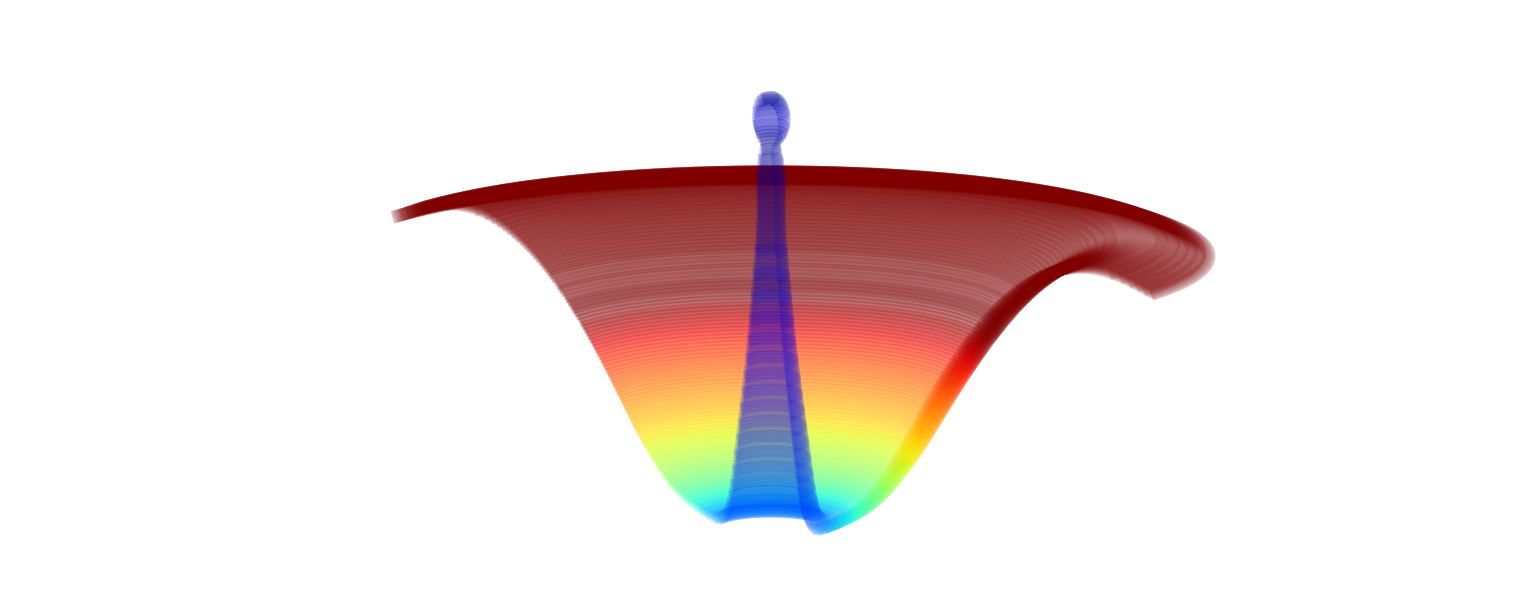
\includegraphics[width=0.75\linewidth]{WriteUp/images/droplet release 3D.png}
    \caption{An image of jet formation due to a burst bubble}
    \label{fig:1}
\end{figure}

Since the pioneering study of bursting bubbles by Woodcock \textit{et al.} \cite{woodcock1953giant}, numerous studies have been made documenting jet drop properties. The first comprehensive study using numerical simulations based on a free-surface formulation of the Navier-Stokes equations was done in 2002 by Duchemin \textit{et al.} \cite{duchemin2002jet
}.

In this paper they used a volume-of-fluid (VOF) type method to investigate quantities such as the jet velocity, maximum pressure on the axis of symmetry and radius of the first ejected drop. They compared their numerical data with experimental data published by MacIntyre \cite{macintyre1972flow} and found the overall agreement satisfactory. The method was able to resolve small capillary wave and still scuratly predict large scale features of the dynamics, the pressure and final droplet radius.

Another aim of this paper was to investigate bubble entrapment. This is when a new bubble is formed underneath the collapsing cavity of the old bubble. Two entrapment regions were found, the first for $576<R/R_v<2016$ and the second between $57\:600<R/R_v<288\:000$ where $R$ is the radius of the bubble and $R_v=\rho\nu^2/\sigma$ is the viscous-capillary length with $\rho$, $\nu$ and $\sigma$ being liquid density, kinematic viscosity and surface tension respectively. Other regions of entrapment at higher values of $R/R_v$ was speculated but was said to be difficult to observe numerically.

Duchemin \textit{et al.} also showed that the jets are produced by the self-similar collapse of a cavity created by capillary waves.
